\section{Auswertung}
\label{sec:Auswertung}

Die Messung der Apparaturkonstanten liefert folgende Werte:
\begin{gather*}
  r_\text{K} = \frac{53,60}{2} \si{\milli\meter} = 0,0268 \si{\meter} \\
  m_\text{K} = 141,97 \si{\gram} = 0,14197 \si{\kilo\gram} \\
  J_\text{K} = \frac{2}{5} m_\text{K} r_\text{K}^2 = 4,1 \cdot 10^{-5} \si{\kilo\gram\meter\squared} \\
  N = 195 \\
  d = 0,138 \si{\meter} \\
  R_\text{Spule} = 0,109 \si{\meter}
\end{gather*}

\subsection{Bestimmung des magnetichen Moments eines Magneten unter Ausnutzung der Gravitation}
Mithilfe von Gleichung (4) wird die Magnetfeldstärke ausgerechnet.
\begin{table}
\centering
\caption{Magnetfeldstärke $B$ in Abhängigkeit von Abstand $r$ und Spulenstrom $I$}
\label{tab:bfeld}
\begin{tabular}{c c c}
\toprule
Abstand $r\:/\:\cdot 10^{-2}\si{\meter}$ & Spulenstrom $I\:/\:\si{\ampere}$ & Magnetfeldstärke $B\:/\:\cdot 10^{-3}\si{\tesla}$ \\
\midrule
4,1 & 1,28 & 1,74 \\
4,9 & 1,49 & 2,02 \\
5,3 & 1,58 & 2,14 \\
5,6 & 1,6 & 2,17 \\
6,1 & 1,78 & 2,41 \\
7,2 & 2 & 2,71 \\
8,0 & 2,19 & 2,97 \\
8,9 & 2,35 & 3,19 \\
9,3 & 2,46 & 3,34 \\
10,1 & 2,64 & 3,58 \\
\bottomrule
\end{tabular}
\end{table}

Um das magnetische Moment der Kugel zu berechnen wird die Magnetfeldstärke $B$ gegen den Abstand 
$r$ aufgetragen und mithilfe linearer Regression in Form von 

\begin{gather*}
y = ax+b, \\~\\
a = \frac{\overline{xy}-\overline x\overline y}{\overline{x^2}-\overline{x}^2} = 0.0303,\\~\\
b = \frac{\overline{x^2}\overline{y}-\overline{x}\overline{xy}}{\overline{x^2}-\overline{x}^2} = 0.0005
\end{gather*}
wird die Steigung der Ausgleichsgeraden bestimmt.

\begin{figure}
  \center
  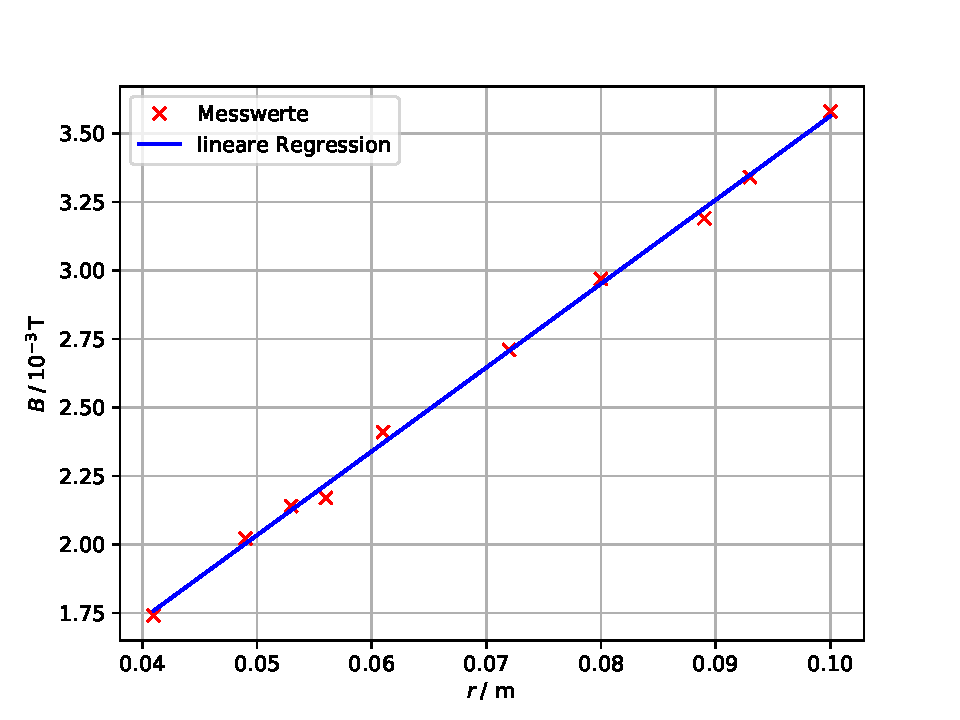
\includegraphics{feldstaerke.pdf}
  \caption{Feldstärke in Abhängigkeit des Abstands}
  \label{fig:feldstaerke}
\end{figure}

Nun wird nach Gleichung (7) das magnetische Moment $\mu_\text{Dipol}$ gemäß
\begin{gather}
\mu_\text{Dipol} = \frac{m_\text{g}g}{a}
\end{gather}
berechnet.
Mit
\begin{gather*}
m_\text{g} = 0,00138 \si{\kilo\gram}, \\
g = 9,81 \si{\meter\per\second\squared}, \\
a = 0,303 \si{\kilo\gram\meter\per\second\squared\per\ampere\per\meter\squared}
\end{gather*}
folgt:
\begin{gather*}
\mu_\text{Dipol1} = 0,447 \,\si{\ampere\meter\squared}.
\end{gather*}

\subsection{Bestimmung des magnetischen Moments über die Schwingungsdauer eines Magneten}
Mittels Gleichung (4) wird erneut die Magnetfeldstärke $B$ der jeweiligen Stromstärke $I$ berechnet.
\begin{table}
\centering
\caption{Zur Stromstärke $I$ zugehörige Magnetfeldstärke $B$ und Periodendauer $T$}
\label{tab:schwingung}
\begin{tabular}{c c c}
\toprule
Spulenstrom $I\:/\:\si{\ampere}$ & Magnetfeldstärke $B\:/\:\cdot 10^{-3}\si{\tesla}$ & Periodendauer $T\:/\:\cdot 10^{-1}\si{\second}$ \\
\midrule
3,8 & 5,15 & 8,46 \\
3,5 & 4,75 & 8,66 \\
3,2 & 4,34 & 8,86 \\
2,9 & 3,93 & 9,54 \\
2,6 & 3,53 & 10,05 \\
2,3 & 3,12 & 10,69 \\
2,0 & 2,71 & 11,45 \\
1,7 & 2,31 & 12,52 \\
1,4 & 1,90 & 13,76 \\
1,1 & 1,49 & 15,61 \\
\bottomrule
\end{tabular}
\end{table}
Um das magnetische Moment $\mu_\text{Dipol}$ zu berechnen wird $T^2$ gegen $1/B$ aufgetragen.
\begin{figure}[H]
  \center
  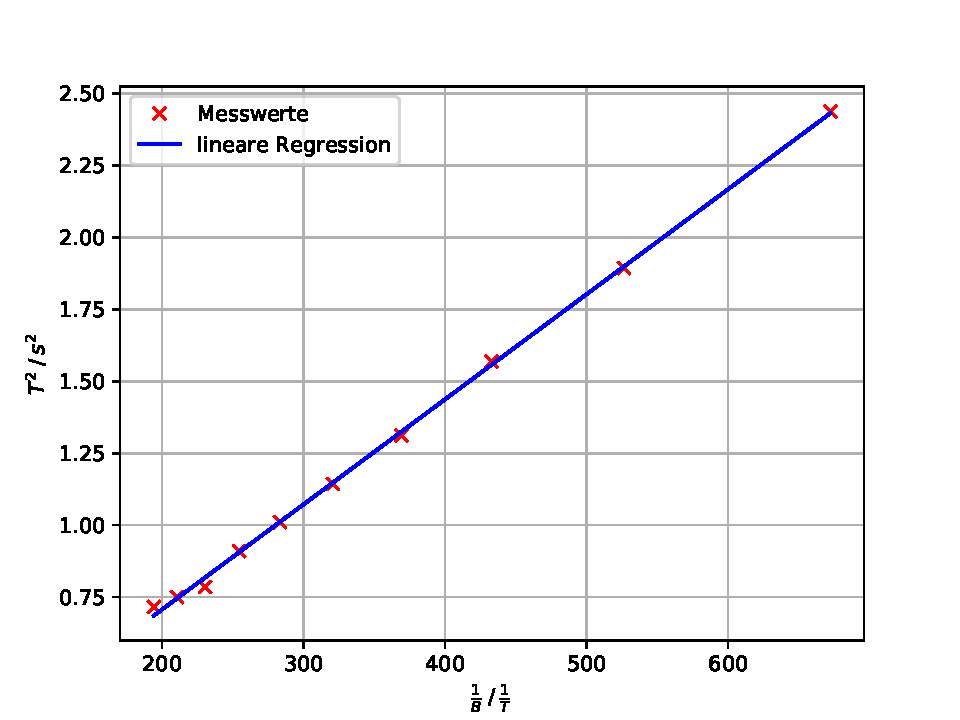
\includegraphics{schwingung.pdf}
  \caption{Schwingungsdauer in Abhängigkeit von der Magnetfeldstärke}
  \label{fig:schwingung}
\end{figure}
Mittels linearer Regression ergibt sich für die Ausgleichsgerade
\begin{gather*}
a = 0,00365, \\
b = -0,023.
\end{gather*}
Aus Gleichung (9) ergibt sich somit für das magnetische Moment
\begin{gather}
\mu_\text{Dipol2} = \frac{4\pi^2J_\text{K}}{a} = 0,443\,\si{\ampere\meter\squared}.
\end{gather}

\subsection{Bestimmung des magnetischen Moments über die Präzession}
Um das magnetische Moment $\mu_\text{Dipol}$ zu bestimmen wird die reziproke Periodendauer $T_\text{P}$
gegen die Magnetfeldstärke $B$ aufgetragen, welche sich aus der Stromstärke $I$ mittels Gleichung (4) ergibt.
\begin{table}
\centering
\caption{Zur Stromstärke $I$ zugehörige Magnetfeldstärke $B$ und reziproke Periodendauer $T_\text{P}$}
\label{tab:praezession}
\begin{tabular}{c c c}
\toprule
Spulenstrom $I\:/\:\si{\ampere}$ & Magnetfeldstärke $B\:/\:\cdot 10^{-3}\si{\tesla}$ & $T_\text{P}\:/\:\si{\second}^{-1}$ \\
\midrule
0,2 & 0,27 & 0,0240 \\
0,5 & 0,68 & 0,0439 \\
0,8 & 1,08 & 0,0593 \\
1,1 & 1,49 & 0,0749 \\
1,4 & 1,90 & 0,0917 \\
1,7 & 2,31 & 0,1205 \\
2,0 & 2,71 & 0,1689 \\
2,3 & 3,12 & 0,1745 \\
2,6 & 3,53 & 0,2160 \\
2.8 & 3,80 & 0,2212 \\
\bottomrule
\end{tabular}
\end{table}
\begin{figure}
  \center
  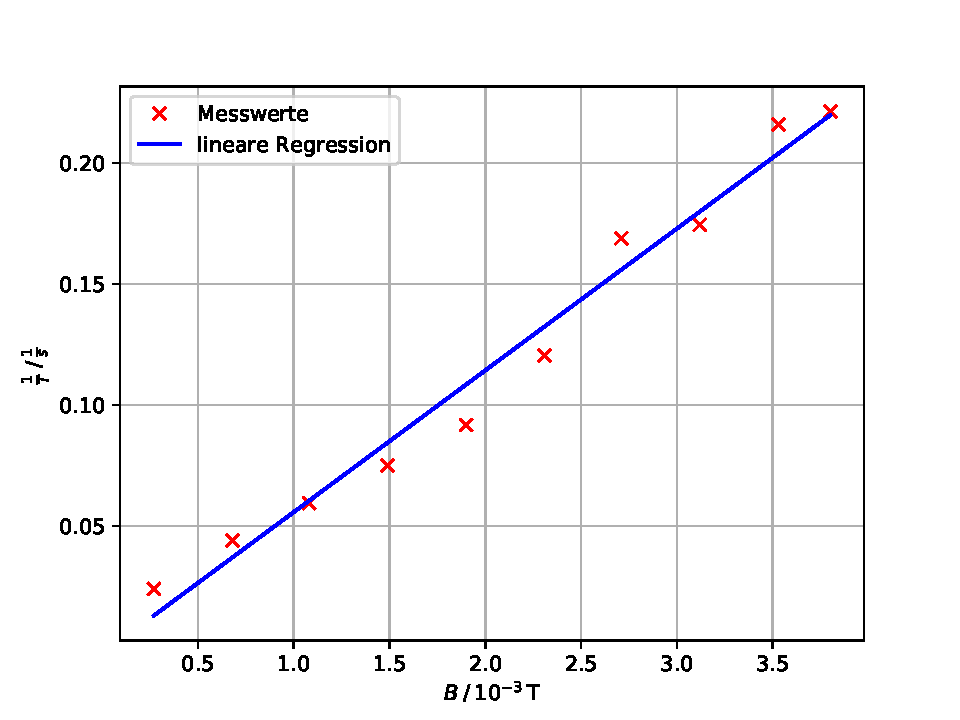
\includegraphics{praezession.pdf}
  \caption{Umlaufzeit in Abhängigkeit von der Magnetfeldstärke}
  \label{fig:praezession}
\end{figure}

Mithilfe der linearen Regression ergibt sich für die Ausgleichsgerade
\begin{gather*}
a = 0,0586, \\
b = -0,003.
\end{gather*}
Aus der Steigung der Geraden lässt sich mittels
\begin{gather}
\mu_\text{Dipol} = 2\pi L_\text{K} a
\end{gather}
mit
\begin{gather*}
L_\text{K} = 4,1 \cdot 10^{-5} \si{\kilo\gram\meter\squared} \cdot 2\pi \cdot 4,3\si{\hertz} = 1,11 \cdot 10^{-3} \si{\kilo\gram\meter\squared\per\second}
\end{gather*}
das magnetische Moment berechnen:
\begin{gather*}
\mu_\text{Dipol3} = 0,453\,\si{\ampere\meter\squared}.
\end{gather*}